\documentclass[11pt]{article}
\usepackage[a4paper, margin=2.54cm]{geometry}
\usepackage[utf8]{inputenc}
\usepackage[spanish, mexico]{babel}
\usepackage[spanish]{layout}
\usepackage[article]{ragged2e}
\usepackage{textcomp}
\usepackage{amsmath}
\usepackage{amssymb}
\usepackage{amsfonts}
\usepackage{enumerate}
\usepackage{graphicx}

% ============================================================================
% ============================================================================
% ============================================================================

\title{
  Entrega N° 1 \\
  \large Modelos Físicos
}
\author{
  Farizano, Juan Ignacio \\
  \and
  Mellino, Natalia \\
  \and
  Prato, Valentina
}
\date{}

% ============================================================================
% ============================================================================
% ============================================================================

\begin{document}

\maketitle
\noindent\rule{\textwidth}{1pt}

\section*{Ejercicio 11.81}

\subsection*{Enunciado}

El registro de aceleración que se muestra en la figura se obtuvo
durante las pruebas de rapidez de un automóvil deportivo. Si se sabe que
el automóvil inicia desde el reposo, determine de manera aproximada:
\begin{enumerate}[a)]
  \item La velocidad del automóvil en $t = 8s$
  \item La distancia recorrida por el automóvil en $t = 20s$
\end{enumerate}

\begin{figure}[h!]
  \begin{center}
    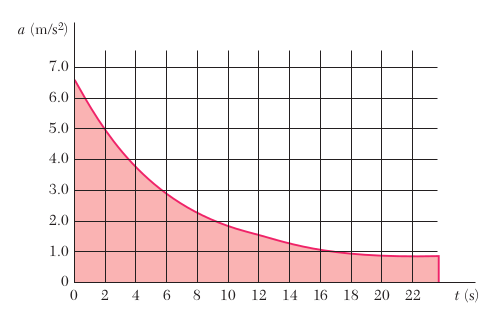
\includegraphics[width=0.75\linewidth]{graficoEnunciado81.png}
  \end{center}
\end{figure}

\subsection*{Resolución}

\subsection*{Apartado a)}
El gráfico está dividido en rectángulos de anchos $\Delta t = t_{k+1}-t_k = 2s$

Sabemos que $v_0 = 0$ y $v_i = v_0 + \displaystyle\sum_{k = 0}^{i - 1} a_p(t_k, t_{k + 1}) \Delta t$ con
$a_p(t_k, t_{k + 1}) = \frac{a(t_k) + a(t_{k+1})}{2} \Rightarrow v_i = 2s \cdot \displaystyle\sum_{k = 0}^{i - 1} a_p(t_k, t_{k + 1})$

Para calcular $v_8$, tenemos que calcular $a_p$ para los intervalos
$(0, 2), (2, 4), (4, 6), (6,8)$

\begin{align*}
  a_p(0, 2) =& \frac{a(0)+ a(2)}{2} \approxeq \frac{6.5m/s^2 + 5m/s^2}{2} = 5.75m/s^2\\
  a_p(2, 4) \approxeq& \frac{5m/s^2 + 3.75m/s^2}{2} = 4.375m/s^2 \\
  a_p(4, 6) \approxeq& \frac{3.75m/s^2 + 3m/s^2}{2} = 3.375m/s^2 \\
  a_p(6, 8) \approxeq& \frac{3m/s^2 + 2.25m/s^2}{2} = 2.625m/s^2 \\
  \Rightarrow v_8 =& 2s \cdot (5.75 + 4.375 + 3.375 + 2.62)m/s^2 = 32.25m/s
\end{align*}

$\therefore$ La velocidad del auto en el tiempo $t = 8s$ es igual a $v_8 = 32.25m/s$

\subsection*{Apartado b)}
También sabemos que $x_i = x_0 + \displaystyle\sum_{k = 0}^{i - 1} v_p(t_k, t_{k + 1}) \Delta t$ con
$v_p(t_k, t_{k + 1}) = \frac{v(t_k) + v(t_{k+1})}{2}$. \\
Para calcular la distancia recorrida hasta los 20s se puede suponer que $x_0 = 0$
y simplemente calcular $x_{20}$.

Para esto se debe calcular $a_p$ para los 10 intervalos de 2s entre 0s y 20s, 
y con esto calcular $v_p$ para cada intervalo. 

El del intervalo siguiente se puede obtener añadiendo el próximo
$a_p\Delta t$ al del intervalo actual.

Sabiendo que $v_0 = 0$ calculamos.

\begin{align*}
  v_2 =& a_p(0, 2) \cdot t = 5.72m/s^2 \cdot 2s = 11.5 m/s
   \Rightarrow v_p(0, 2) = \frac{v_0 + v_2}{2} = 5.75m/s \\
  v_4 =& v_2 + a_p(2, 4) \cdot t = 11.5m/s + 4.375m/s^2 \cdot 2s = 20.25m/s
   \Rightarrow v_p(2, 4) = 15.875m/s \\
  v_6 =& 27m/s \Rightarrow v_p(4, 6) = 23.625m/s \\
  v_8 =& 32.25m/s \Rightarrow v_p(6, 8) = 29.625m/s \\
  a_p(8, 10) =& \frac{2.25m/s^2 + 1.75m/s^2}{2} = 2m/s^2
   \Rightarrow v_{10} = 36.25m/s \Rightarrow v_p(8, 10) = 34.25m/s \\
  a_p(10, 12) =& \frac{1.75m/s^2 + 1.5m/s^2}{2} = 1.625m/s^2
   \Rightarrow v_{12} = 39.5m/s \Rightarrow v_p(10, 12) = 37.875m/s \\
  a_p(12, 14) =& \frac{1.5m/s^2 + 1.25m/s^2}{2} = 1.375m/s^2
   \Rightarrow v_{14} = 42.25m/s \Rightarrow v_p(12, 14) = 40.875m/s \\
  a_p(14, 16) =& \frac{1.25m/s^2 + 1m/s^2}{2} = 1.125m/s^2
   \Rightarrow v_{16} = 44.5m/s \Rightarrow v_p(14, 16) = 43.375m/s \\
  a_p(16, 18) =& \frac{1m/s^2 + 1m/s^2}{2} = 1m/s^2
   \Rightarrow v_{18} = 46.5m/s \Rightarrow v_p(16, 18) = 45.5m/s \\
  a_p(18, 20) =& \frac{1m/s^2 + 0.75m/s^2}{2} = 0.875m/s^2
   \Rightarrow v_{20} = 48.25m/s \Rightarrow v_p(18, 20) = 47.375m/s \\
\end{align*}

\begin{align*}
  x_{20} &= 0 + 2s \cdot (5.75 m/s &+ 15.875m/s + 23.625m/s + 29.625m/s + 34.25m/s + 37.875m/s + 40.875m/s \\
         &                         &+ 43.375m/s + 45.5m/s + 47.375m/s) \\
         &= 648.25m
\end{align*}

$\therefore$ La distancia recorrida por el automóvil en el tiempo $t = 20s$
es igual a $x_{20} = 648.25m$

% ============================================================================
% ============================================================================
% ============================================================================

\section*{Ejercicio 11.100}

\subsection*{Enunciado}

Una máquina lanzadora “dispara” pelotas de béisbol con una
velocidad horizontal $v_0$ . Si se sabe que la altura $h$ varía entre $31$ in. y $42$ in.,
determine:
\begin{enumerate}[a)]
  \item El rango de valores de $v_0$.
  \item Los valores de $\alpha$ correspondientes a $h = 31$ in. y $h = 42$ in.
\end{enumerate}

\begin{figure}[h!]
  \begin{center}
    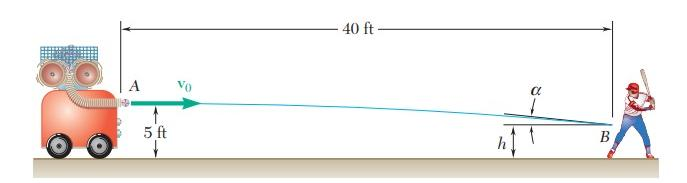
\includegraphics[width=0.99\linewidth]{graficoEnunciado100.jpeg}
  \end{center}
\end{figure}

% ============================================================================

\subsection*{Resolución}

Para resolver el problema, primero fijamos nuestro sistema de referencia.
Situamos el origen en el punto A donde parte la pelota. El eje $x$ es positivo
hacia la derecha, y el eje $y$ es positivo hacia abajo. \\

Recordemos las siguientes ecuaciones que nos serán de utilidad:
\begin{equation}
  \label{eq:v100}
  v(t) = v_0 + a \cdot t
\end{equation}
\begin{equation}
  \label{eq:x100}
  x(t) = x_0 + v_0 \cdot t + \frac{1}{2} \cdot a \cdot t^2 
\end{equation}

Ahora trabajamos por separado para cada valor de $h$ \\
 
$\bullet$ $h = 31in = 2.58ft$:

Tenemos entonces que nuestra \textbf{posición inicial} es $(0, 0)$ y nuestra
\textbf{posición final} será dada por $(40, 5 - h) = (40, 2.42)$. Ahora, 
queremos hallar nuestro vector de velocidad inicial $v_0 = ((v_x)_0, (v_y)_0)$.
Podemos deducir que el valor para $(v_y)_0$ es $ (v_y)_0 = 0 ft/s$.
Luego, con este dato, podemos usar la ecuación \ref{eq:x100} y despejar el tiempo $t$ en $y$:

\begin{align*}
  y(t) &= y_0 + (v_y)_0 \cdot t + \frac{1}{2} \cdot a \cdot t^2 \\
  2.42ft &= 0 + 0 + \frac{1}{2} \cdot g \cdot t^2 \\
  2.42ft &= \frac{1}{2} \cdot (32.17ft/s^2) \cdot t^2 \\
  2.42ft &= 16.085ft/s^2 \cdot t^2  \\
  \frac{2.42ft}{16.085ft/s^2} &= t^2 \\
  0.387s &= t
\end{align*}

Entonces se tiene que el tiempo que tarda la pelota en llegar al final de su
recorrido es $t = 0.387s$. Ahora, podemos reemplazar este valor en la ecuación \ref{eq:x100}
y despejar la $(v_x)_0$ para $x$.

\begin{align*}
  40ft &= 0 + (v_x)_0 \cdot (0.387s) + \frac{1}{2} \cdot 0 \cdot t^2 \\
  40ft &= (v_x)_0 \cdot (0.387s) \\
  103.359ft/s &= (v_x)_0
\end{align*}

Por lo tanto, hallamos que $v_0 = (103.359, 0)$. \\

Ahora queremos hallar nuestro ángulo $\alpha$. Recordemos que:
\begin{equation}
  \label{eq:modx100}
  \vert v_f \vert \cdot \cos \alpha = (v_x)_f
\end{equation}
\begin{equation}
  \label{eq:mody100}
  \vert v_f \vert \cdot \sin \alpha = (v_y)_f  
\end{equation}

Donde $v_f$ es nuestro vector de velocidad final y debemos hallar sus componentes.
Como la velocidad en $x$ siempre es constante, tenemos que $(v_x)_f = 103.359 ft/s$.
Para hallar la $(v_y)_f$ utilizamos la ecuación \ref{eq:v100} y sustituimos $t$ por el 
tiempo final, asi obtenemos la velocidad final.

\begin{align*}
  v_y(t) &= (v_y)_0 + a \cdot t \\
  v_y(t) &= 0 + (32.17ft/s^2) \cdot 0.387s \\
  v_y(t) &= 12.44ft/s
\end{align*}

Ahora, calculamos $\vert v_f \vert = \vert (103.359, 12.44) \vert = \sqrt{103.359^2 + 12.44^2} = 104.104$. \\

Reemplazando en la ecuación \ref{eq:modx100}, podemos despejar $\alpha$:

\begin{align*}
  104.104ft/s \cdot \cos \alpha &= 103.359ft/s \\
   \cos \alpha &= \frac{103.359ft/s}{104.104ft/s} \\
   \cos \alpha &= 0.992 \\
   \alpha &= \arccos 0.992 \\
   \alpha &= 0.126rad
\end{align*}

$\bullet$ $h = 42in = 3.5ft$

El razonamiento es completamente análogo, solamente hay que reemplazar los valores de $h$.

\begin{itemize}
  \item Posición inicial: (0, 0)
  \item Posición final: $(40, 5-3.5) - (40, 1.5)$
  \item $(v_0)_y = 0$
\end{itemize}

Despejamos el tiempo $t$ para $y$ en la ecuación \ref{eq:x100}:

\begin{align*}
  1.5ft &= \frac{1}{2} \cdot (32.17ft/s^2) \cdot t^2 \\
  1.5ft &= 16.085ft/s^2 \cdot t^2  \\
  \frac{1.5ft}{16.085ft/s^2} &= t^2 \\
  0.305s &= t
\end{align*}

Reemplazamos el valor de $t$ en la ecuación de $x(t)$ y hallamos $(v_x)_0$:
\begin{align*}
  40ft &= 0 + (v_x)_0 \cdot (0.305s) + \frac{1}{2} \cdot 0 \cdot t^2 \\
  40ft &= (v_x)_0 \cdot (0.305s) \\
  131.147ft/s &= (v_x)_0
\end{align*}

Para hallar el ángulo $\alpha$ seguimos el mismo procedimiento que antes.
Hallamos $v_f$: tenemos que $(v_x)_f = 131.147 ft/s$, pues en $x$ la velocidad es constante.
Para hallar la $(v_y)_f$ utilizamos la ecuación \ref{eq:v100} y sustituimos $t$ por el 
tiempo final, asi obtenemos la velocidad final.
\begin{align*}
  v_y(t) &= (v_y)_0 + a \cdot t \\
  v_y(t) &= 0 + (32.17ft/s^2) \cdot 0.305s \\
  v_y(t) &= 9.811ft/s
\end{align*}

Luego: $v_f = (131.147, 9.811) \Rightarrow \vert v_f \vert = \sqrt{131.147^2 + 9.811^2} = 131.513$ \\

Finalmente utilizando la ecuación \ref{eq:modx100}:
\begin{align*}
  131.513ft/s \cdot \cos \alpha &= 131.147ft/s \\
   \cos \alpha &= \frac{131.147ft/s}{131.513ft/s} \\
   \alpha &= \arccos 0.997 \\
   \alpha &= 0.074rad
\end{align*}

Por todo lo analizado anteriormente podemos concluir que:

\begin{enumerate}[a)]
  \item El rango de valores de $v_0$ es $103.359f t/s \leq v_0 \leq 131.147f t/s$ 
  \item Los valores de $\alpha$ para $h = 31in$ y $h = 42in$ son $\alpha = 0.126rad$ 
        y $\alpha = 0.074rad$ respectivamente.
\end{enumerate}

% ============================================================================
% ============================================================================
% ============================================================================

\section*{Ejercicio 11.153}

\subsection*{Enunciado}

Un satélite viajará de manera indefinida en una órbita circular alrededor de un
planeta si la componente normal de la aceleración del satélite es igual
a $g{(\frac{R}{r})}^2$, donde $g$ es la aceleración de la gravedad
en la superficie del planeta, $R$ es el radio del planeta, y $r$ es la distancia desde
el centro del planeta al satélite. Determine la rapidez de un satélite relativa
al planeta indicado, si el satélite se desplaza de manera indefinida en una órbita
circular a 160 km sobre la superficie del planeta.

\subsection*{Resolución}

El planeta dado es Venus. Luego:

\begin{equation*}
  g = 8.53m/s^2, R = 6161km \Rightarrow r=160km + R = 6321km
\end{equation*}

Del enunciado sabemos que la componente normal de la aceleración $a_n$ es
$a_n = g{(\frac{R}{r})}^2$ y por teoría sabemos que $a_n = \frac{v^2}{r}$.
A partir de esto, despejamos $v$:

\begin{align*}
  a_n &= \frac{v^2}{r} = g \frac{R^2}{r^2} \Rightarrow v^2 = g \frac{R^2}{r} \\
  \Rightarrow v &= R\sqrt{\frac{g}{r}} \\
  &= 6161km \cdot \sqrt{\frac{8.53m/s^2}{6321km}} \\
  &= 6161000m \cdot \sqrt{\frac{8.53m/s^2}{6321000m}} \\
  &= \frac{6161000m}{860.9s} \\
  &= 7156.46 m/s \\
  &= 25763.26km/h
\end{align*}

$\therefore$ Por lo tanto la rapidez de un satélite relativa a Venus estando
en órbita circular a 160km sobre la superficie del planeta es igual a 
$v = 25763.26km/h$

\end{document}